Linking items and in general finding similarity among these already area-specific texts proved to be a problematic task. To test my algorithm I've decided to compare 89 SO questions with its matching Git issue and one more random git issue of the project. Results 




Although I wasn't successful to such extent that the output are Git-StackOverflow or Git-Reddit pairs, I've pointed out some interesting results and data relationships.

\subsection{Stack Overflow}
The average similarity between SO questions talking about particular issue and that particular issue (using NLTK approach) description is 0.316 without body preprocessing and 0.292 with body preprocessing.

The distribution of similarities in buckets by increased by 0.05 can be seen in histogram in Figure \ref{fig:GitStackMatchesHistogram}

\begin{figure}[H]%
    \centering
	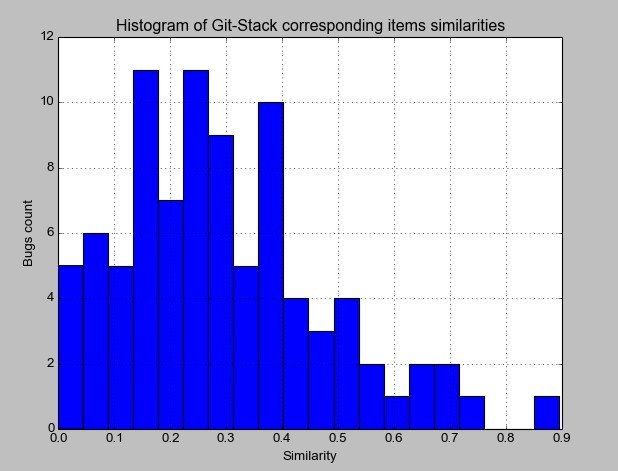
\includegraphics[width=8cm]{gitStackMatchesHistogram.jpg}
    \caption{Histogram of similarities distribution among git issues and their matching SO questions}%
    \label{fig:GitStackMatchesHistogram}%
\end{figure}

For random SO questions, amount of comparisons to Git issues needed to be limited. If every SO question would be compared to every Git issue, time of computation would exceed timeframe of this thesis. Every SO question was therefore compared to 20 random git issues and resulting average similarity scores are in following figures.

\begin{figure}[H]%
    \centering
	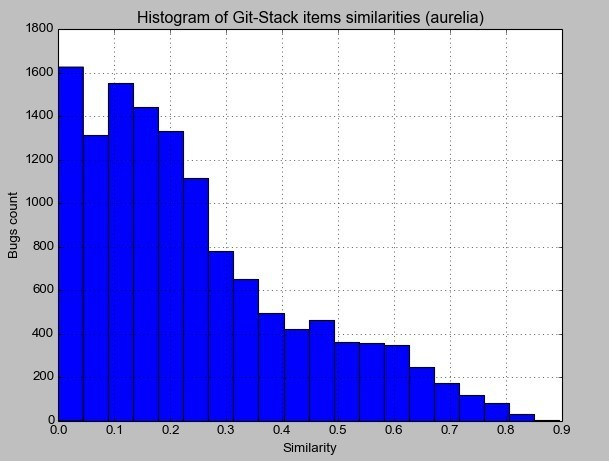
\includegraphics[width=8cm]{AureliaStackWithRandom20Bugs.jpg}
    \caption{Histogram of Aurelia SO questions and random git issues. Average similarity was 0.244}%
    \label{fig:AureliaStackWithRandom3Bugs}%
\end{figure}

\begin{figure}[H]%
    \centering
    \subfloat[EmberJS average similarity - 0.247]{{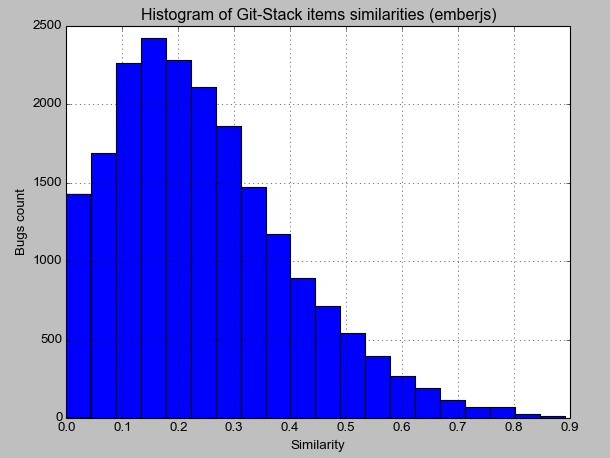
\includegraphics[width=6cm]{EmberStackWithRandom20Bugs.jpg} }}%
    \qquad
    \subfloat[Bower average similarity - 0.217]{{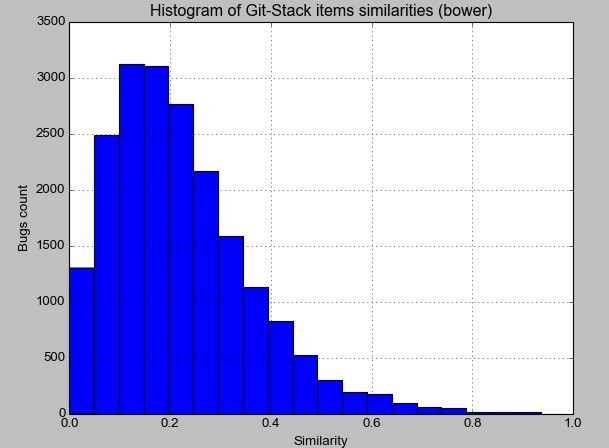
\includegraphics[width=6cm]{BowerStackWithRandom20Bugs.jpg} }}%
    \caption{EmberJS and Bower similarity histogram}%
    \label{fig:BowerEmberWithRandom3Bugs}%
\end{figure}

\begin{figure}[H]%
    \centering
    \subfloat[VueJS average similarity - 0.255]{{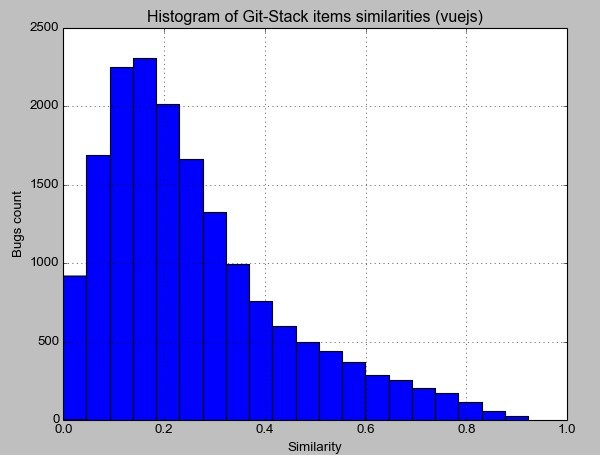
\includegraphics[width=6cm]{VueJSStackWithRandom20Bugs.jpg} }}%
    \qquad
    \subfloat[AngularJS average similarity - 0.258]{{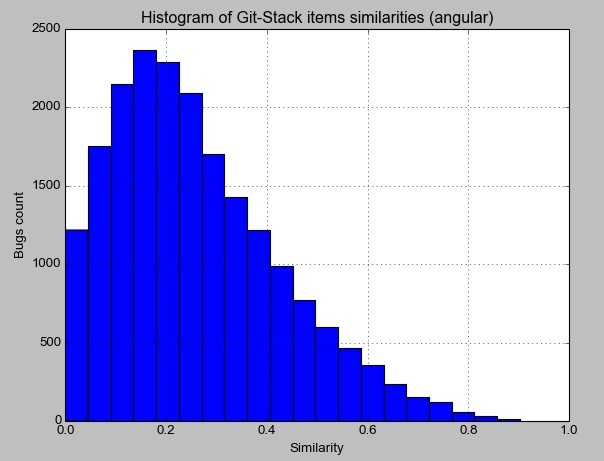
\includegraphics[width=6cm]{AngularStackWithRandom20Bugs.jpg} }}%
    \caption{VueJS and AngularJS similarity histogram}%
    \label{fig:VueAngularWithRandom3Bugs}%
\end{figure}


Table \ref{table:StackOverflowNLTKsimilarity} illustrates results of comparing Git bugs descriptions with SO questions talking about own project issues and general issues. From values displayed, it's apparent that the difference between matches and random pairs is not very big. This is probably because all the texts about a particular project are already very specific and similar in their nature anyway.

\begin{table}[H]
\centering
\begin{tabular}{ |p{3cm}||p{4.5cm}|p{5.5cm}|}
 \hline
\textbf{ Framework }& \textbf{Own issues similarity}& \textbf{20 random issues similarity}\\
 \hline
 NodeJS   & 0.265 & 0.243\\ \hline
 AngularJS & 0.241 & 0.260\\ \hline
 EmberJS & 0.282 & 0.246\\ \hline 
 VueJS &   0.261 & 0.258\\ \hline
\end{tabular}
\caption{NLTK similarity values for SO questions}
\label{table:StackOverflowNLTKsimilarity}
\end{table}

\subsection{Reddit}Here I've calculated the similarity between the bug description and either particular comment in the reddit discussion which mentioned the bug or the whole discussion itself. Using NLTK BOW approach, average similarity score for all considered projects (NodeJS, AngularJS, VueJS and EmberJS) was 0.481 for the whole discussion and 0.368 for the comment itself. Scikit If-Idf values were 0.263 and 0.207 respectively. Detailed scores for each project can be found in table \ref{table:RedditNLTKsimilarity} for NLTK implementation and  table for \ref{table:RedditSCIKITsimilarity}. Subreddit for EmberJS didn't reference any of its own bugs.

\begin{table}[H]
\centering
\begin{tabular}{ |p{3cm}||p{3cm}|p{4cm}|}
 \hline
\textbf{ Framework }& \textbf{Bug comment}& \textbf{Whole discussion}\\
 \hline
 NodeJS   & 0.447 & 0.507\\ \hline 
 AngularJS & 0.306 & 0.57 \\ \hline 
 VueJS &   0.359 & 0.380\\ \hline
\end{tabular}
\caption{Reddit NLTK similarity values}
\label{table:RedditNLTKsimilarity}
\end{table}

\begin{table}[H]
\centering
\begin{tabular}{ |p{3cm}||p{3cm}|p{4cm}|}
 \hline
\textbf{ Framework }& \textbf{Bug comment}& \textbf{Whole discussion}\\
 \hline
 NodeJS   & 0.255 & 0.328\\ \hline 
 AngularJS & 0.168 & 0.278 \\ \hline 
 VueJS &  0.209  & 0.208\\ \hline
\end{tabular}
\caption{Reddit Scikit similarity values}
\label{table:RedditSCIKITsimilarity}
\end{table}

Both similarity calculations indicate that the semantic meaning of the bug is better expressed in the whole discussion rather than just the particular comment which referenced the bug. This made me question if it could be generalized that longer the text is, more similar it is to actual bug description. I've plotted a relationship between similarity score and length in Figures \ref{fig:SimilarityLengthRelationshipComment} and \ref{fig:SimilarityLengthRelationshipDiscussion}.

\begin{figure}[H]%
    \centering
	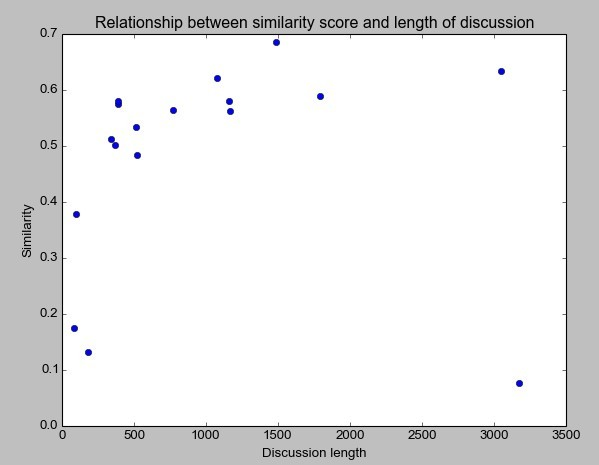
\includegraphics[width=8cm]{SimilarityLengthRelationshipDiscussion.jpg}
    \caption{Discussion lengths and similarity scores with the issue}%
    \label{fig:SimilarityLengthRelationshipDiscussion}%
\end{figure}

\begin{figure}[H]%
    \centering
	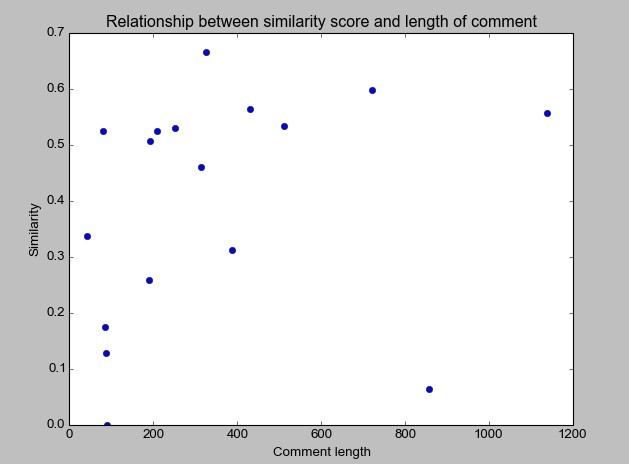
\includegraphics[width=8cm]{SimilarityLengthRelationshipComment.jpg}
    \caption{Comment lengths and similarity scores with the issue}%
    \label{fig:SimilarityLengthRelationshipComment}%
\end{figure}


